\documentclass[11pt, a4paper, french]{article}
\usepackage{lmodern}
\usepackage{babel}
\usepackage[utf8]{inputenc}
\usepackage[T1]{fontenc}
\usepackage[margin = 2.5 cm]{geometry}
\usepackage{graphicx}   % Insertion des images
\usepackage{tocloft}    % Personnalisation de la table des matières
\usepackage{parskip}    % Facultatif : permet de retirer les alinéas et surtout d'espacer les paragraphes
\usepackage{fancyhdr}   % Personnalisation des en-têtes et pieds de page

\pagestyle{fancy}

% IMPORTANT
% Variable pour définir si l'on souhaite utiliser les parties (\part{...}). Par défaut, on ne les utilise pas.
% Cela change notamment la structuration de la table des matières.
\newif\ifUseParts
\UsePartsfalse % ou \UsePartstrue

% ------------------------------------------------------------------------------------------------------------
% Si on utilise les parties, on définit les règles applicables à la table des matières
\ifUseParts
  % On définit les règles applicables à la table des matières en prenant en compte les parties
  \counterwithin*{section}{part}
  \renewcommand\thepart{\arabic{part}.}
  \renewcommand\thesection{\arabic{part}.\arabic{section}.}
  \renewcommand\thesubsection{\arabic{part}.\arabic{section}.\arabic{subsection}.}
  \renewcommand\thesubsubsection{\arabic{part}.\arabic{section}.\arabic{subsection}.\arabic{subsubsection}.}
\else
  % On redéfinit la numérotation des sections pour qu'elle ne prenne pas en compte les parties
  \renewcommand\thesection{\arabic{section}.}
  \renewcommand\thesubsection{\arabic{section}.\arabic{subsection}.}
  \renewcommand\thesubsubsection{\arabic{section}.\arabic{subsection}.\arabic{subsubsection}.}
\fi

% Table des matières
\setcounter{tocdepth}{2}                    % Nombre max de niveau dans la table des matières

\setlength{\cftbeforesecskip}{0.50 em}      % Espacement avant les titres des sections
\setlength{\cftsecindent}{2.25 em}          % Espacement entre la marge le numéro des sections
\setlength{\cftsecnumwidth}{2.25 em}        % Espacement entre le titre des sections et le numéro

\setlength{\cftbeforesubsecskip}{0.25 em}   % Espacement avant les titres des sous-sections
\setlength{\cftsubsecindent}{4.5 em}        % Espacement entre la marge le numéro des sous sections
\setlength{\cftsubsecnumwidth}{2.875 em}    % Espacement entre le titre de la section et le numéro des sous sections

% Pour aligner les points de la table des matières
\makeatletter
\renewcommand{\cftdotfill}[1]{
  \def\@tempa{#1}
  \def\@tempb{\cftnodots}
  \ifx\@tempa\@tempb
  \hfill
  \else
  \leaders\hbox to 2.25 mm{\hss\cftdot\hss}\hskip 4mm plus1fill
  \fi
}
\makeatother

\renewcommand{\headrulewidth}{0pt}
\setlength{\footskip}{40 pt}
\setlength{\headheight}{50 pt}
\setlength{\voffset}{-20pt}

% Pour pouvoir écrire au-dessus d'une page où \maketitle est présent
\fancypagestyle{plain}{
  \fancyhf{}
  \renewcommand{\headrulewidth}{0pt}
  \fancyhead[L]{
      
\includegraphics[height = 12 mm]{Images/Logos/Logo.PoPS.pdf}
  }

  \fancyhead[R]{
      
\includegraphics[height = 12 mm]{Images/Logos/Logo.UPS.pdf}
  }

  \fancyfoot[L] {
      \noindent\makebox[\textwidth]{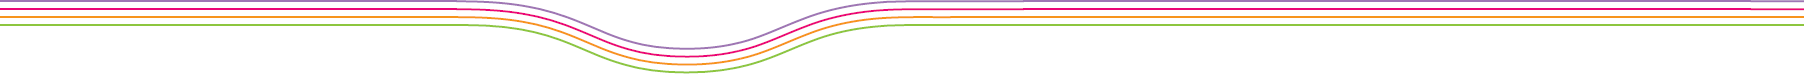
\includegraphics[width=\paperwidth]{Images/Polytech/Lignes.png}}
  }
}

% Règles applicables à toutes les pages sauf la première
\fancyfoot[C]{ \thepage }
\fancyhead[] { \fancyhf }

\title  {\textbf{Cours / TD / TP}\\Nom du module    }
\author {Cours par P\up{r}. X Y                     }
\date   {Année 20XX - 20YY                          }

\begin{document}

\maketitle

\tableofcontents

\newpage

\section{Première section}
Lorem ipsum dolor sit amet, consectetur adipiscing elit. Donec eleifend ultricies maximus. Phasellus sed dolor semper nulla pellentesque vulputate. Cras ac massa elit. Etiam in nisl vitae turpis dignissim iaculis.

\subsection{Première sous-section}
Sed hendrerit arcu magna, eget maximus nunc lobortis at. Nullam lacinia est sit amet neque varius, non rhoncus velit condimentum. Sed fringilla blandit pharetra. Aliquam in sem purus. Quisque in nunc id erat sagittis luctus non quis leo. Curabitur blandit erat a sem pulvinar, in consequat ipsum luctus. Nulla posuere nunc non purus pellentesque semper. Sed malesuada convallis dolor quis tristique. 

\subsubsection{Première sous-sous-section}
Phasellus tempus, quam eu laoreet rhoncus, ipsum diam dapibus diam, eget tincidunt risus risus vitae nulla. Nullam nec sem sed leo dapibus venenatis at vitae tortor. Suspendisse rhoncus non eros a sagittis. Fusce vel elit pellentesque, sollicitudin felis vel, imperdiet sem. Aenean nisi odio, fringilla ac scelerisque commodo, finibus id mauris.

\section{Deuxième section}
Lorem ipsum dolor sit amet, consectetur adipiscing elit. Donec eleifend ultricies maximus. Phasellus sed dolor semper nulla pellentesque vulputate. Cras ac massa elit. Etiam in nisl vitae turpis dignissim iaculis.

\subsection{Deuxième sous-section}
Sed hendrerit arcu magna, eget maximus nunc lobortis at. Nullam lacinia est sit amet neque varius, non rhoncus velit condimentum. Sed fringilla blandit pharetra. Aliquam in sem purus. Quisque in nunc id erat sagittis luctus non quis leo. Curabitur blandit erat a sem pulvinar, in consequat ipsum luctus. Nulla posuere nunc non purus pellentesque semper. Sed malesuada convallis dolor quis tristique. 

\subsubsection{Deuxième sous-sous-section}
Phasellus tempus, quam eu laoreet rhoncus, ipsum diam dapibus diam, eget tincidunt risus risus vitae nulla. Nullam nec sem sed leo dapibus venenatis at vitae tortor. Suspendisse rhoncus non eros a sagittis. Fusce vel elit pellentesque, sollicitudin felis vel, imperdiet sem. Aenean nisi odio, fringilla ac scelerisque commodo, finibus id mauris.

\end{document}